\documentclass[12pt]{article}
\usepackage{tikz}
\usepackage{ifthen}
\usetikzlibrary{arrows}

% type, redundancy, required, lambda 
\newcommand{\modelgraphlabel}[4]{$#1$ \\ $r=#2$ \\ $\nu=#3$ \\ $\lambda=#4$}

\begin{document}
% Cloud Model 
% draw - outline, fill - color!alpha, align - allows for manual linebreak
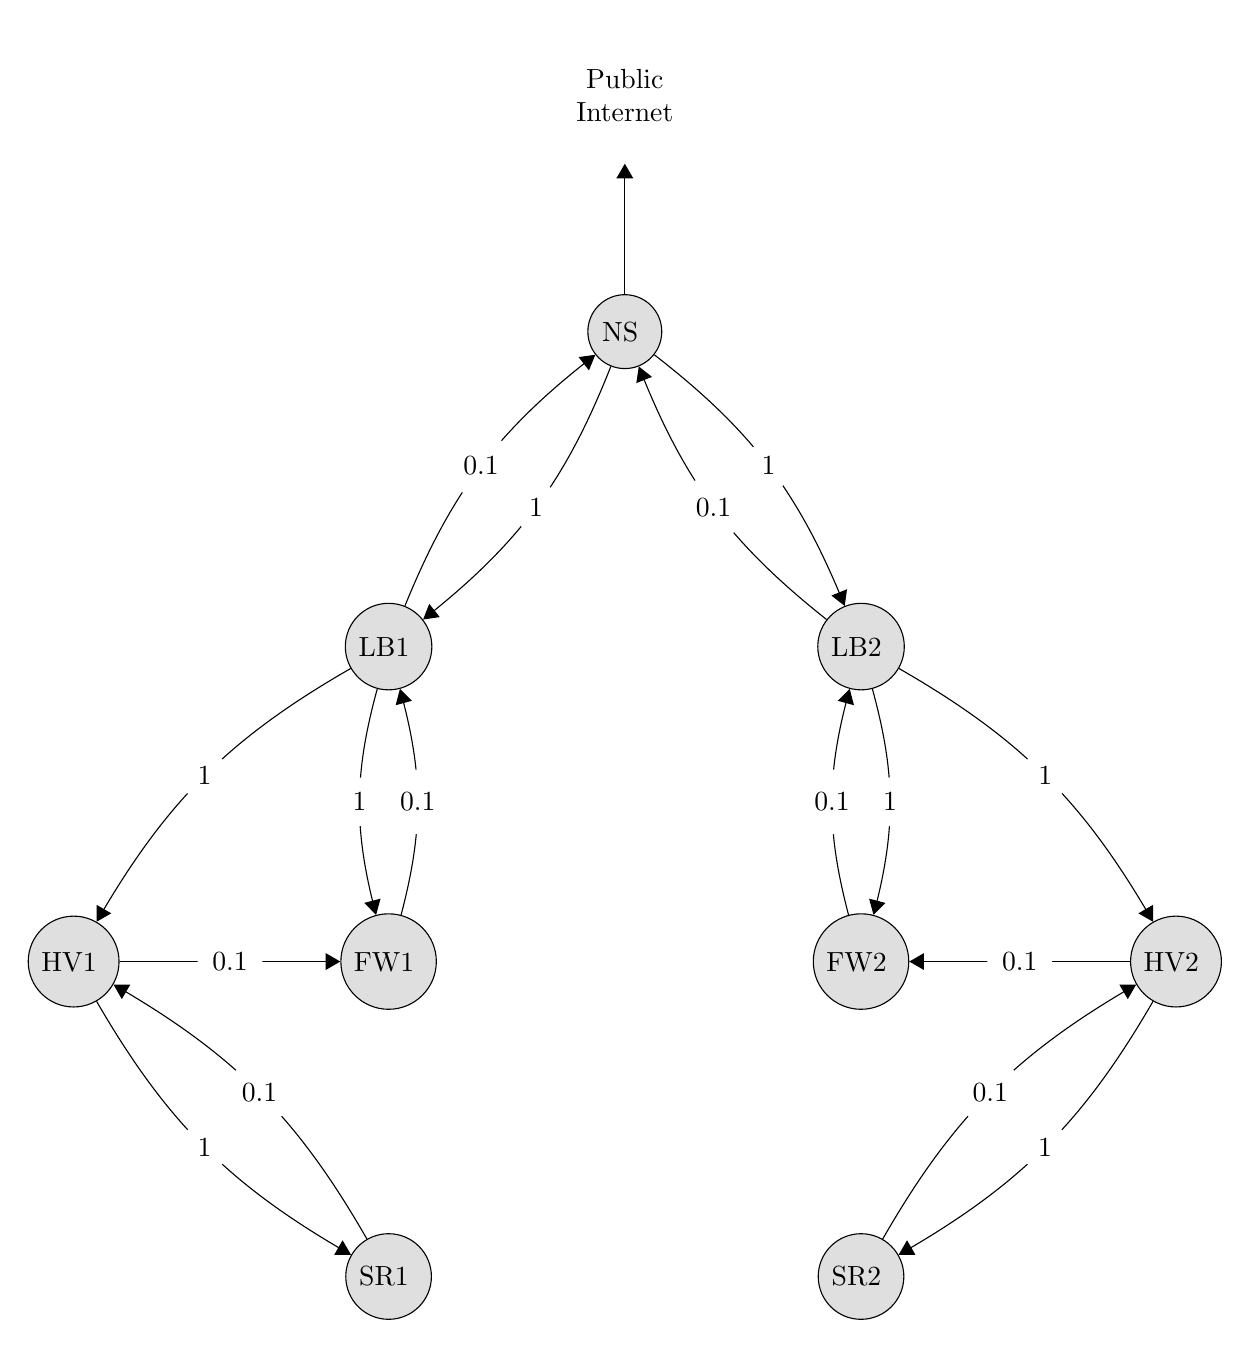
\begin{tikzpicture}[scale = 1, auto = center, every node/.style = {circle, draw = black, fill = gray!25}, bend angle = 90]

	\node (NS)  at ( 0, 16) [align = center] {\iffalse \modelgraphlabel{NS}  {2}{1} {0.01} \fi {NS}  };
	\node (LB1) at (-3, 12) [align = center] {\iffalse \modelgraphlabel{LB1} {2}{1} {0.01} \fi {LB1} };
	\node (LB2) at ( 3, 12) [align = center] {\iffalse \modelgraphlabel{LB2} {2}{1} {0.01} \fi {LB2} };
	\node (FW1) at (-3,  8) [align = center] {\iffalse \modelgraphlabel{FW1} {2}{1} {0.01} \fi {FW1} };  
	\node (FW2) at ( 3,  8) [align = center] {\iffalse \modelgraphlabel{FW2} {2}{1} {0.01} \fi {FW2} };
	\node (HV1) at (-7,  8) [align = center] {\iffalse \modelgraphlabel{HV1} {2}{1} {0.01} \fi {HV1} };
	\node (HV2) at ( 7,  8) [align = center] {\iffalse \modelgraphlabel{HV2} {2}{1} {0.01} \fi {HV2} };  
	\node (SR1) at (-3,  4) [align = center] {\iffalse \modelgraphlabel{SR1} {3}{2} {0.01} \fi {SR1} };
	\node (SR2) at ( 3,  4) [align = center] {\iffalse \modelgraphlabel{SR2} {3}{2} {0.01} \fi {SR2} };
	\node (PB)  at ( 0, 19) [align = center, fill=none, draw=none] {Public\\Internet};

    \foreach \from/\phy/\to in {NS/1/LB1, NS/1/LB2, LB1/0.1/NS, LB2/0.1/NS, 
    LB2/1/FW2, FW2/0.1/LB2, LB2/1/HV2, SR2/0.1/HV2, HV2/1/SR2}
    	\path (\from) edge [-triangle 60, bend left = 15] node[fill=white, draw=none] {\phy} (\to);
    \foreach \from/\phy/\to in {LB1/1/FW1, FW1/0.1/LB1, LB1/1/HV1, SR1/0.1/HV1, HV1/1/SR1}
    	\path (\from) edge [-triangle 60, bend right = 15] node[fill=white, draw=none] {\phy} (\to);
    \foreach \from/\phy/\to in {HV1/0.1/FW1, HV2/0.1/FW2}
    	\path (\from) edge [-triangle 60] node[fill=white, draw=none] {\phy} (\to);

    \path (NS) edge [-triangle 60] node[fill=none, draw=none] {} (PB);

\end{tikzpicture}

\newpage

We now consider a model representing a cloud computing architecture. Our system is designed to handle Hyper Text Transfer Protocol (HTTP) requests and Simple Mail Transfer Protocol (SMTP) requests. NS represents a Network Switch; LB1, 2 represent two types of Load Balancers; FW 1, 2 represent two types of firewalls; HV 1, 2 represent two types hypervisors and SR 1, 2 represent two types of server racks. This organization of components specifically shows a firewall ``sandwich" as described in \cite{Salch:2004}. 

We set $r_{NS} = r_{LB1} = r_{LB2} = r_{FW1} = r_{FW2} = r_{HV1} = r_{HV2} = 2$ and $r_{SR1} = r_{SR2} = 3$. We need at least two server racks of both types SR 1, 2 to be up to be able to parallel process across server racks. For other component types, we require at least one component of each type of the system up in order for the system to remain operational. Thus, $\upsilon_{NS} = \upsilon_{LB1} = \upsilon_{LB2} = \upsilon_{FW1} = \upsilon_{FW2} = \upsilon_{HV1} = \upsilon_{HV2} = 1$ and $\upsilon_{SR1} = \upsilon_{SR2} = 2$. Additionally, our system operates in two environments - high demand and low demand. This gives us a state space of size 69984. Traditionally solving a model of this size using DECAF1 would take a very long time whereas using DECAF2's tree generation algorithms given in section \ref{sec:alg} it takes xxxx seconds. 

We build the system such that all component types that are located to the left of network switch (i.e. types with a 1 in their name) handle SMTP requests only whereas all component types located to the right of the network switch (i.e types with a 2 in their name) handle HTTP requests only. Thus both the branches need to be operational for the system to be able to handle HTTP and SMTP requests.

We assume that failure of any component causes a certain, downward propagating, cascading failure because components have no option but to go offline and reach a dormant state. To comply with our model dormancy is treated as a failure.        

\bibliographystyle{plain}
\bibliography{cloud} 

\end{document}